\subsection{Limiting Amplitude and Limiting Absorption Principle}
In this section we perform several numerical experiments,
with the normalization chosen as $\epsilon_0=\mu_0=1$, $\omega=c=1$. 
Also, we set $m_e=1$ and $e=-1$. From this it follows that $w_c=-B_0$ and $w_p^2=N_e$. 
We consider the following two cases:
\begin{itemize}
 \item case $N_e\neq \operatorname{const}$, no resonance;
 \item case $N_e\neq \operatorname{const}$, resonance.
\end{itemize}
For every fixed absorption rate $\nu$, in the time domain we choose the boundary conditions of the form
\begin{align}
\label{eq:bcs}
\left.\partial_t H\right|_{x=-L}&=-\left.\partial_x E_y\right|_{x=-L}=G\sin(t),\; G\in \mathbb{R}, \\
 \nonumber
 \left.\partial_t H\right|_{x=H}&=0,
\end{align}
and zero initial conditions, and in the frequency domain
\begin{align*}
 \left.\partial_x \hat{E}_y\right|_{x=-L}&=G,\\
 \left.\partial_x \hat{E}_y\right|_{x=H}&=0.
\end{align*}
We compute the solution $\mathbf{E}^{\nu}(t)$ for large $t$ in the time domain (the solution computed numerically at the time step $n$ is denoted by $\mathbf{E}^{\nu}_{n}$), and the solution $\hat{\mathbf{E}}^{\nu}$ in the frequency domain. 
In the numerical experiments we check whether the following two quantities
\begin{align*}
\lim_{t\rightarrow+\infty}\mathbf{E}^{\nu}(t), \text{ and } \Im\left(\hat{\mathbf{E}}^{\nu}\exp(it)\right)
\end{align*}
are close as $\nu\rightarrow 0$ (provided that the first of these quantities exists). 
\subsubsection{No-Resonance Case}
We choose the parameters so that in the frequency domain, for the limiting amplitude problem, $\hat{E}_{y}$ satisfies 
the Airy equation. 

We set $\omega_c=0$ (thus $\delta(x)=0$), $\omega=1$ (hence $\alpha(x)=1-N_e(x)$), 
choose the domain as $(-0.5, 10)$ and set the electron density $N_e(x)=1+x$. Importantly, $N_e(x)>0$ on the whole interval.
The boundary conditions in (\ref{eq:bcs}) are chosen as $G=Ai'(0.5)$. 
In all the experiments in this section the CFL number=0.5.


First we set $\nu=10^{-2}$. To demonstrate that the limiting amplitude principle indeed holds, we fix a point $x=x_c$ 
inside the domain and plot the dependence of the solution $E_{y}^{\nu}(x_c,t), \; \Im\left(\hat{E}_y^{\nu}(x_c)\mathrm{e}^{it}\right)$ 
on time $t$ for a range of $t\gg 1$ in Figure \ref{fig:nu1e2_harmon}.  

\begin{figure}[htb]
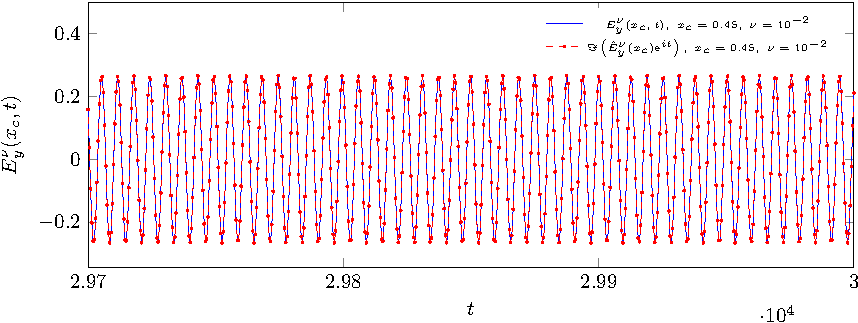
\includegraphics[width=0.9\textwidth]{airy/figure_nu1e2-crop.pdf}
\caption{Dependence of the solution $E_{y}^{\nu}(x_c,t)$ on time for $t\rightarrow +\infty$.}
 \label{fig:nu1e2_harmon}
\end{figure}

In Figure \ref{fig:nu1e2_harmon2} (left figure) we compare this solution to the computed $\hat{E}_y^{\nu}\mathrm{e}^{it}$, for
fixed values of $t$. Both solutions appear to be in close agreement. 
\begin{figure}[htb]
 \begin{tabular}{cc}
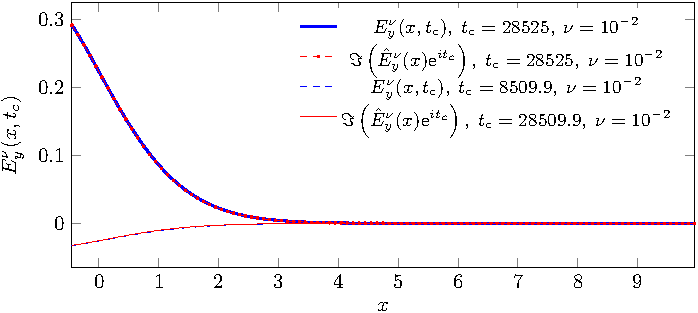
\includegraphics[width=0.5\textwidth]{airy/figure_nu1e2_2-crop.pdf}
&
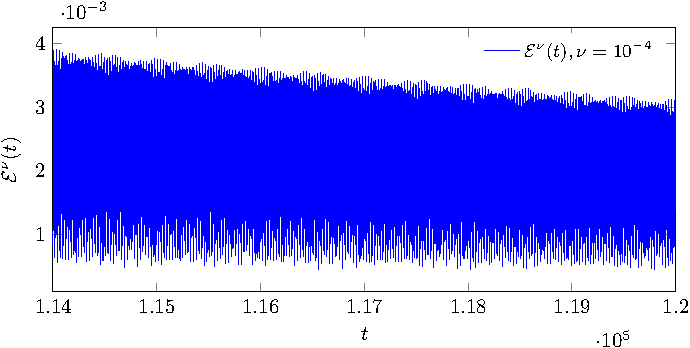
\includegraphics[width=0.5\textwidth]{airy/figure_error_nu1e4-crop.pdf}\\
\end{tabular}
\caption{In the left figure we show the solution for $\nu=10^{-2}$, for two fixed moment of times. In the right figure 
the dependence of the error (\ref{eq:error}) on time for $\nu=10^{-4}$ is demonstrated. 
We can see that the error is decreasing on the given time interval.}
 \label{fig:nu1e2_harmon2}
\end{figure}
\FloatBarrier
The computed $L_2$ error
\begin{align}
\label{eq:error}
\mathcal{E}_{x,y}(t)=\|\Im\left(\hat{E}_{x,y}^{\nu}\exp(it)\right)-E_{x,y}^{\nu}(t)\|_{L_{y}(-L;H)}.
\end{align}
for $\nu=10^{-2}$ did not exceed 1.1e-3 for values of $t\in \left(28501,  30000\right)$. 

Figure \ref{fig:nu1e4_harmon} (left) shows the solutions at a fixed point in space for $\nu=1e-4$. As previously, 
to demonstrate that the limiting amplitude principle indeed holds, we fix a point $x=x_c$ 
inside the domain and plot 
the dependence of the solution $E_{y}^{\nu}(x_c,t)$ on time $t$ for a range of $t\gg 1$. 
The error (\ref{eq:error}) for $\nu=1e-4$ at the time interval $[228000.05,\; 240000.05]$ does not exceed 2.8e-4. 
One of our observations was that for smaller $\nu$ one requires more time steps to achieve the limiting amplitude solution, 
c.f. e.g. Figure \ref{fig:nu1e2_harmon2}. 
For $\nu=10^{-4}$ we were not able to obtain the limiting amplitude solution for $t<3\cdot 10^{4}$, unlike in the case of $\nu=10^{-2}$, 
see also Figure \ref{fig:nu1e2_harmon2}(right). 
For example, for $\nu=10^{-6}$ we were not able to reach the limiting amplitude solution even on the time interval $t\leq 1.92e6$, 
see Figure \ref{fig:nu1e4_harmon} (right). 
\begin{figure}
\begin{tabular}{cc}
 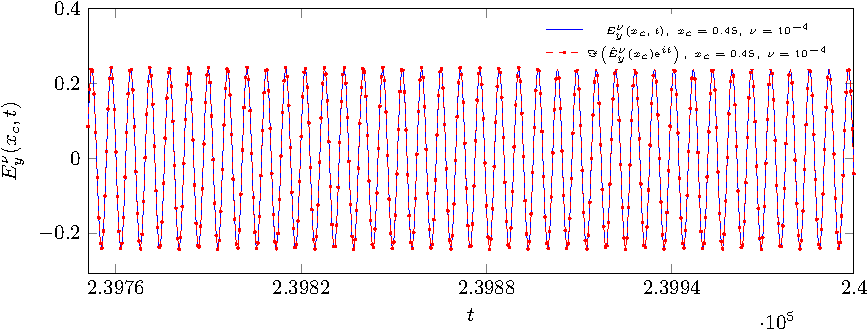
\includegraphics[width=0.5\textwidth]{airy/figure_nu1e4-crop.pdf}&
 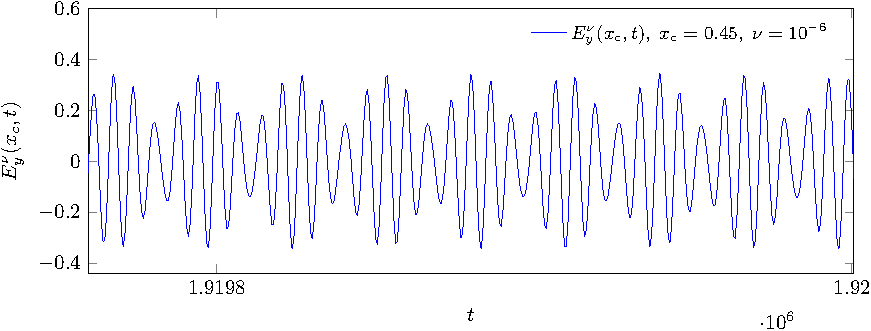
\includegraphics[width=0.5\textwidth]{airy/figure_nu1e6-crop.pdf}\\
\end{tabular}
\caption{In the upper figure we plot the dependence of the solution $E_{y}^{\nu}(x_c,t)$ on time $t$, with $\nu=10^{-4}$ and $x_c=0.45$. 
In the lower figure we show the solution for $\nu=10^{-6}$ at the same point $x_c$, for larger times. As we can see, for 
$\nu=10^{-4}$ the limiting amplitude solution was reached for large $t$. For $\nu=10^{-6}$ we were not able 
to obtain the limiting amplitude solution even for $t\approx 1.9e6$. }
  \label{fig:nu1e4_harmon}
\end{figure}

\subsubsection{Resonance Case}
\label{sec:resn}
For the resonance case, we choose the parameters as in Table \ref{tab:parameters_resonance}.
\begin{table}[htb!]
\begin{tabular}{c|c}
Parameter & Value \\
\hline
$L$ & 5\\
$H$ & 19\\
$\omega_c$ &  \mrev{$\sqrt{0.5}$}\\
$N_e(x)$ &  $\left\{
 \begin{array}{cc}
  0.25, & x<-0.5,\\
  \frac{1+x}{2}, & x\geq -0.5, x\leq 9\\
  5, & x>9.
 \end{array}\right.$\\
 $G$ as in (\ref{eq:bcs}) & 0.11 \\
\end{tabular}
\caption{Parameters for numerical simulations in Section \ref{sec:resn}}
\label{tab:parameters_resonance}
\end{table}
Since $\alpha(x)=(1-2N_e(x))$, $\alpha(0)=0$, and clearly, $\delta(0)\neq 0$.

We compare the results for $\nu=10^{-2},\; 10^{-3}$ in Figures \ref{fig:resonance_nus_ex_x}, 
\ref{fig:resonance_nus_ey_x}, \ref{fig:resonance_nus_ex_t}, \ref{fig:resonance_nus_ey_t}. 
%In the time domain, we chose the discretization size $\Delta x=0.025$. 
The harmonic dependence of the solution on time is demonstrated by fixing $x_c$ inside the domain and plotting 
$E_x^{\nu}(x_c,t)$ and $E_y^{\nu}(x_c, t)$ for a range of $t$. We compare these solutions to $\Im\left(\hat{E}_x^{\nu}(x_c)\mathrm{e}^{it}\right)$ and 
$\Im\left(\hat{E}_y^{\nu}(x_c)\mathrm{e}^{it}\right)$. In the former case we choose the point $x_c=0$, where the resonance occurs. 


\begin{figure}
\begin{tabular}{cc}
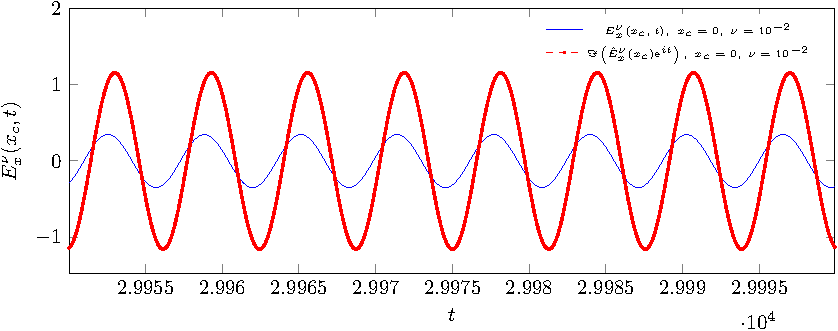
\includegraphics[width=0.5\textwidth]{res/ex_fixed_x-crop.pdf}&
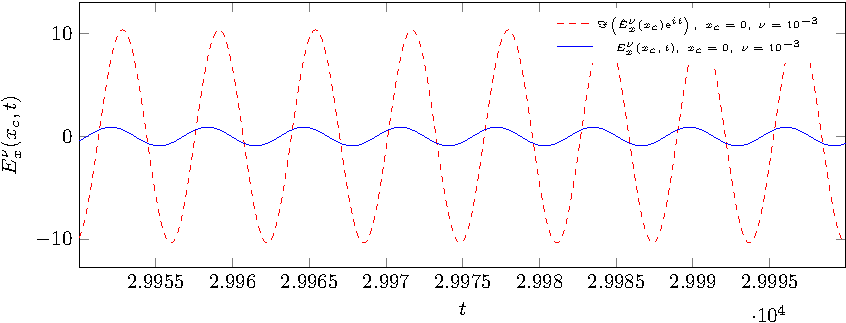
\includegraphics[width=0.5\textwidth]{res/ex_fixed_x_1e3-crop.pdf}
\end{tabular}
\caption{The figures demonstrate the dependence of the solutions 
$E_x^{\nu}(0,t)$ on time $t$ for different values of $\nu$. }
\label{fig:resonance_nus_ex_x}
\end{figure}
\begin{figure}
\begin{tabular}{cc}
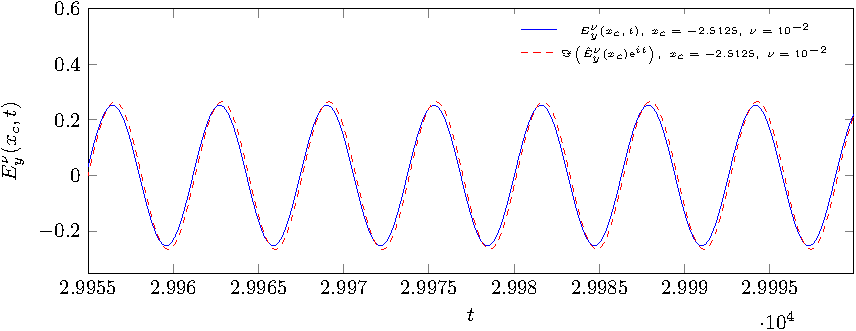
\includegraphics[width=0.5\textwidth]{res/ey_fixed_x-crop.pdf}&
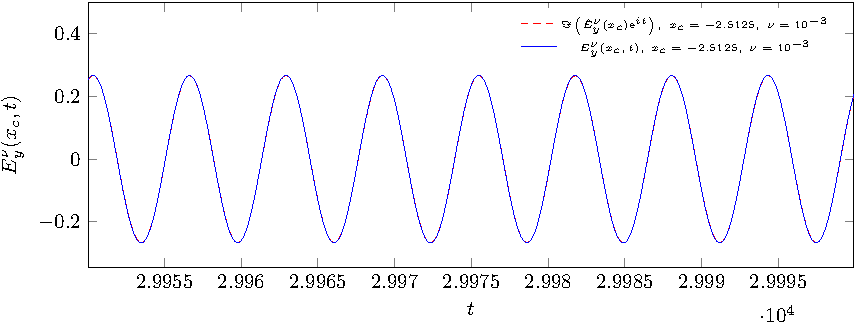
\includegraphics[width=0.5\textwidth]{res/ey_fixed_x_1e3-crop.pdf}
 \end{tabular}
\caption{The figures demonstrate the dependence of the solutions 
$E_y^{\nu}(-2.5125,t)$ on time $t$ for different values of $\nu$. }
\label{fig:resonance_nus_ey_x}
\end{figure}

\begin{figure}
\begin{tabular}{cc}
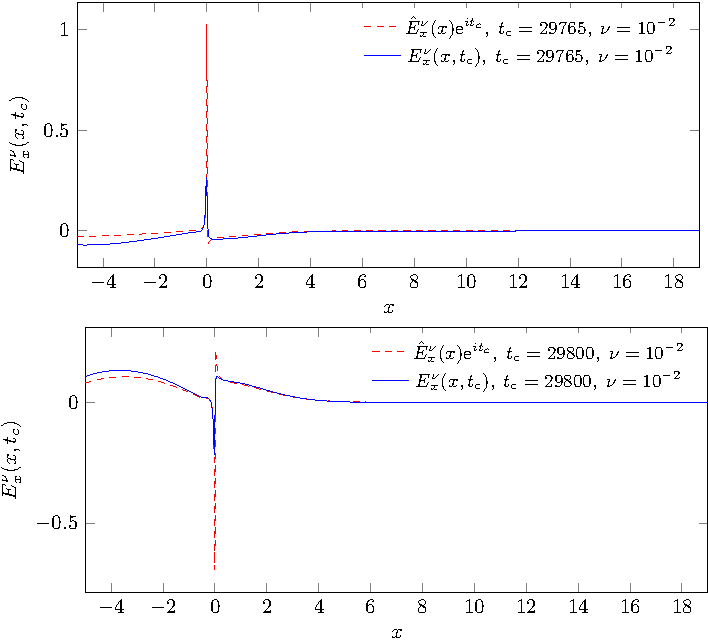
\includegraphics[width=0.5\textwidth]{res/ex_fixed_t-crop.pdf}&
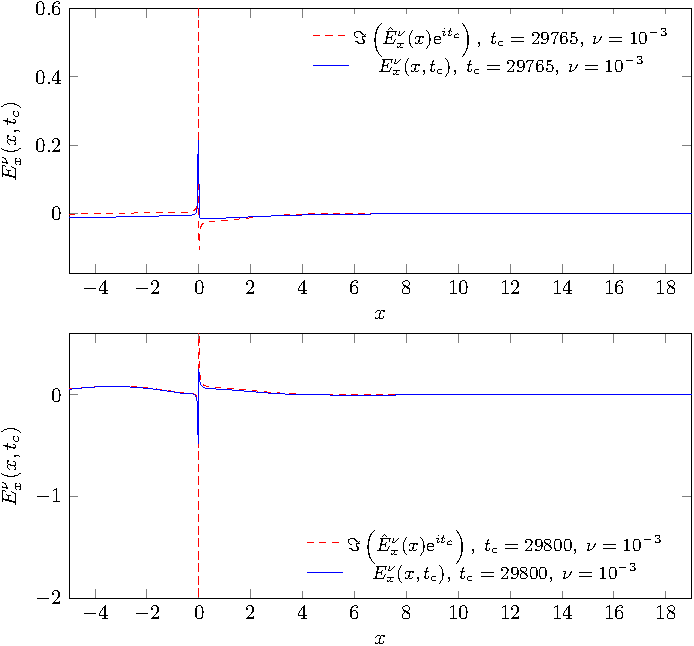
\includegraphics[width=0.5\textwidth]{res/ex_fixed_t_1e3-crop.pdf}
\end{tabular}
\caption{The figures demonstrate the dependence of the solutions 
$E_y^{\nu}(x,t)$ on $x$ for fixed values of $t$. }
\label{fig:resonance_nus_ex_t}
\end{figure}
\begin{figure}
\begin{tabular}{cc}
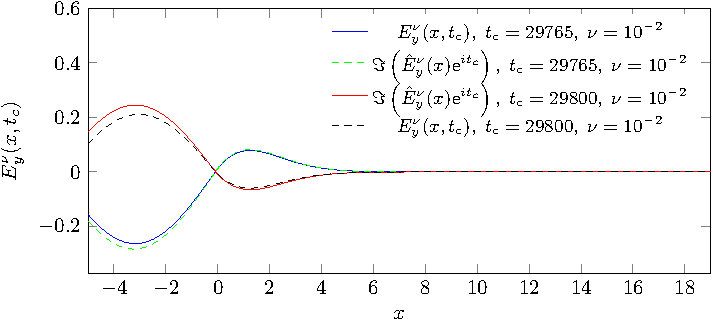
\includegraphics[width=0.5\textwidth]{res/ey_fixed_t-crop.pdf}&
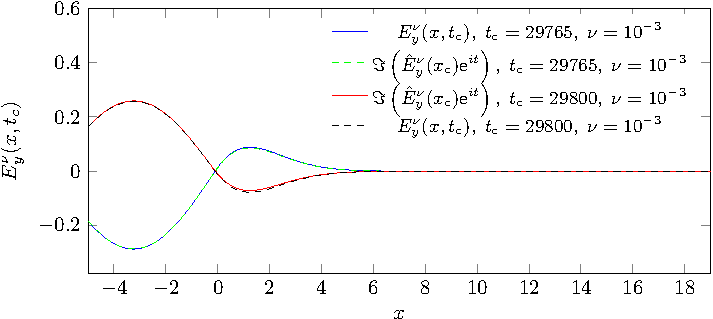
\includegraphics[width=0.5\textwidth]{res/ey_fixed_t_1e3-crop.pdf}
 \end{tabular}
\caption{The figures demonstrate the dependence of the solutions 
$E_y^{\nu}(x,t)$ on $x$ for fixed values of $t$. }
\label{fig:resonance_nus_ey_t}
\end{figure}

We can see that in the case of the resonance, the solution seem to achieve the limiting amplitude solution, 
and both solutions are in relatively close agreement (but the point where the resonance occurs). 
Similarly to the case with the regular case, 
longer computations are needed to achieve the limiting amplitude solution  
for smaller $\nu$.

